\documentclass{article}
\usepackage{graphicx} % Required for inserting images
\usepackage[spanish]{babel}
\usepackage{amsmath}
\usepackage{amsthm}
\usepackage{amssymb}
\usepackage{ dsfont }
\usepackage{adjustbox}
\usepackage[shortlabels]{enumitem}
\usepackage[margin=1in]{geometry}
\usepackage{caption}
\usepackage[nocheck]{fancyhdr}
\usepackage{listings}
\usepackage{hyperref}
\usepackage[
  backend=biber,
  style=apa,
  sortcites=true,
  sorting=nyt,     % orden: autor, año, título
  maxcitenames=2,  % "Autor & Autor (Año)" y luego "Autor et al."
  mincitenames=1,
  maxbibnames=99,
  minbibnames=1,
  maxsortnames=99,
  minsortnames=1,
  giveninits=true, % iniciales en nombres
  url=true, doi=true, isbn=false, eprint=false
]{biblatex}

\usepackage{ragged2e}
\usepackage{setspace} % <-- importante
\doublespacing        % <-- activa doble interlineado
\setlength{\RaggedRightParindent}{\parindent}

% \pagecolor{black} % DarkMode
% \color{white}     % DarkMode

\thispagestyle{fancy}
\rhead{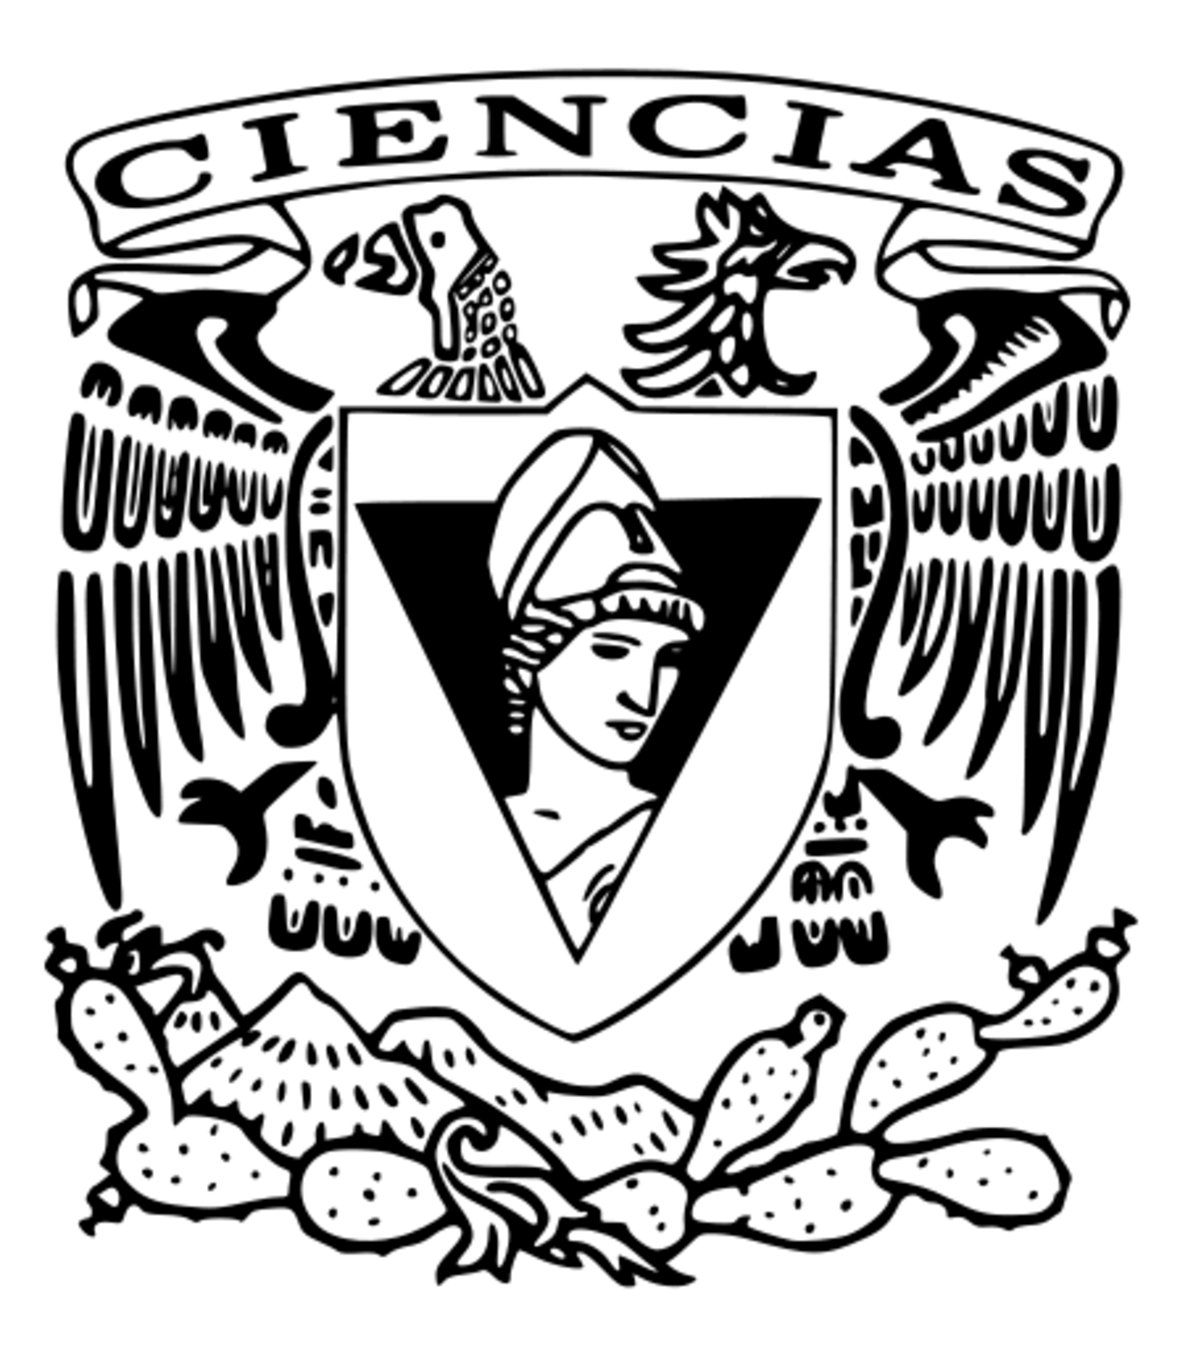
\includegraphics[scale=0.07]{images/Logo_FC.png}}
\lhead{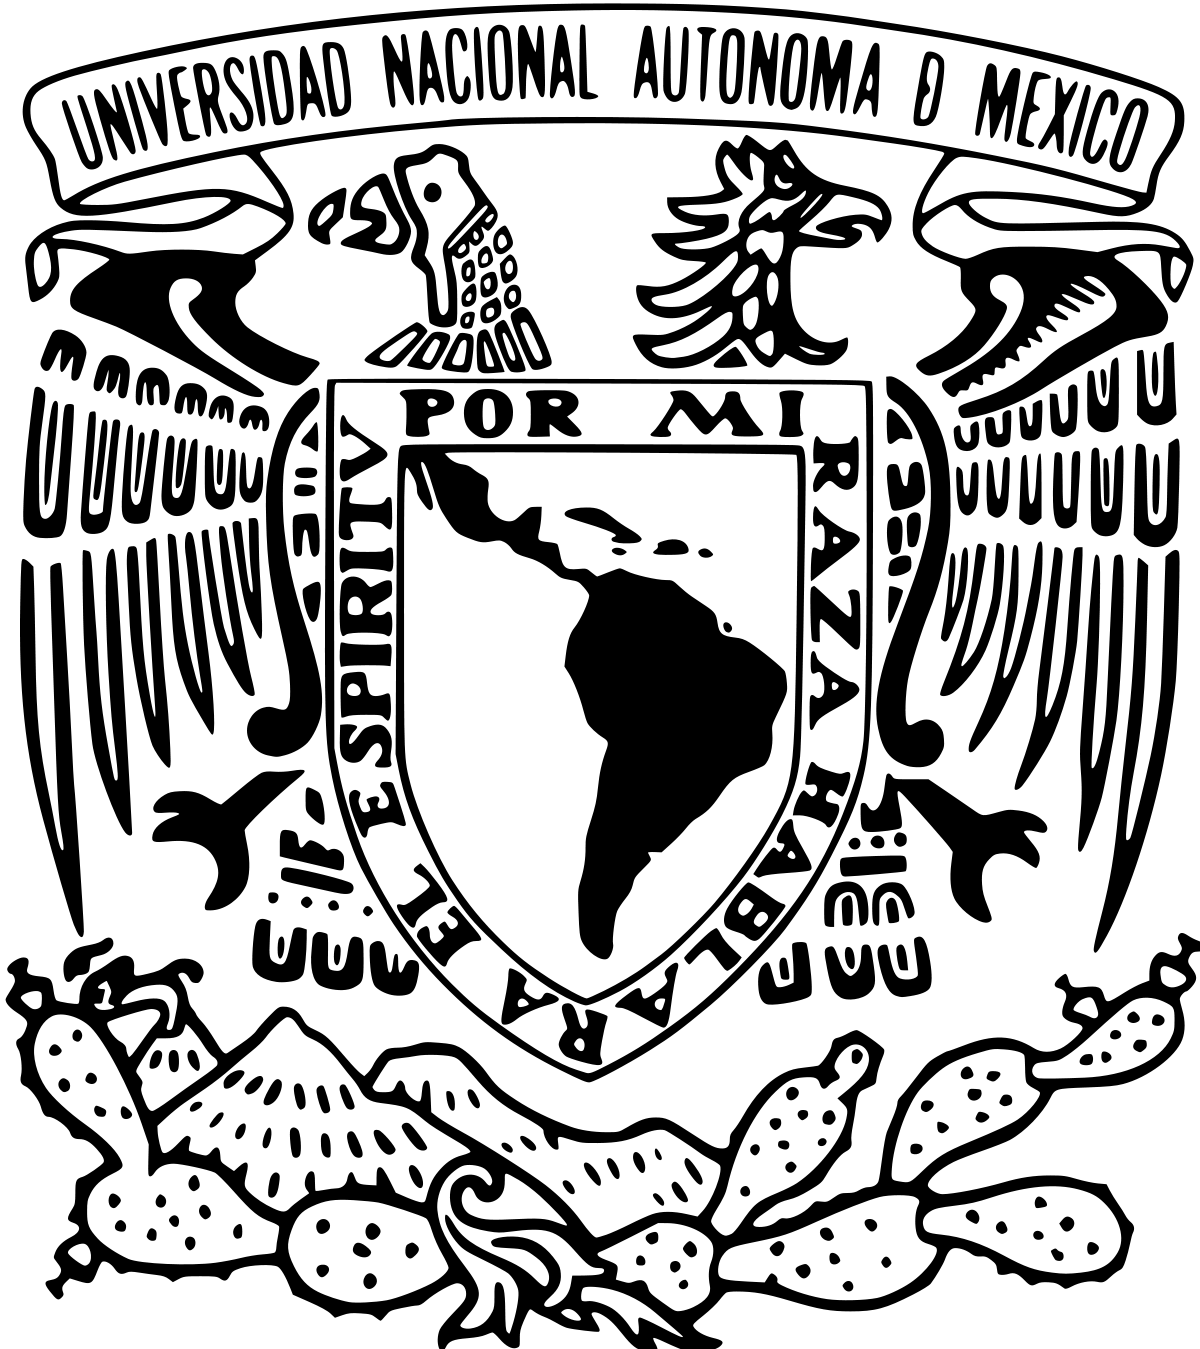
\includegraphics[scale=0.065]{images/Logo_UNAM.png}}
\chead{\large\textbf{Universidad Nacional Autónoma de México} \\
\textbf{Facultad de Ciencias}\\
\textsc{Anexo para titulación por tesis} \\
\textbf{Alumno}: Rodríguez Dimayuga Laura Itzel \\
\textbf{Asesor}: M. en Fil. C. Enrique Francisco Soto Astorga }
\renewcommand{\headrulewidth}{1pt}
\pagenumbering{gobble}
\AtBeginDocument{\vspace*{2\baselineskip}}

\addbibresource{references.bib}
\begin{document}
\section{Título tentativo}
Visualización de patrones de fallo de inferencias causales en grandes 
modelos de lenguaje.

\section{Objetivo}

Establecer un marco teórico que integra la noción de causalidad de \textcite{rosen2012anticipatory}, 
la jerarquía causal de \textcite{pearl2009causality} y el principio ICM de \textcite{scholkopf2021toward}, para demostrar 
que los LLMs operan exclusivamente en el nivel asociativo y carecen de la 
representación mecanística que exige una relación de modelado legítima.

\subsection{Objetivo Secundario}

Validar empíricamente el marco teórico mediante el análisis de los patrones de fallo 
de los LLMs en el benchmark CLadder \parencite{jin2023cladder}. Construyendo un DAG para la visualización 
que evidencie que dichos fallos no son aleatorios sino estructuralmente 
concentrados en los niveles de intervención y contrafactuales, consistentemente con la ausencia de representación 
mecanística predicha por el marco teórico.

\section{Hipótesis}

La hipótesis central sostiene que los grandes modelos de lenguaje (LLMs) no 
son capaces de realizar inferencia causal genuina, sino que operan exclusivamente 
en el nivel de las asociaciones estadísticas, el primer escalón de la jerarquía causal de Pearl.

\section{Pregunta Central}

¿Satisfacen los grandes modelos de lenguaje los criterios requeridos para generar modelos 
causales, o producen únicamente asociaciones estadísticas?

\section{Justificación}

Nuestra capacidad de razonar acerca del mundo y entenderlo viene de encontrar las relaciones de causa y efecto a partir
de la experiencia \parencite{rosen2012anticipatory,pearl2009causality}. Esta capacidad de establecer relaciones causales y 
lógicas entre los eventos del mundo se distingue cualitativamente del 
asociativismo estadístico \parencite{penn2007causal}, y su ausencia en los sistemas de inteligencia 
artificial ha sido señalada como una limitación estructural fundamental.

A medida que el aprendizaje de máquinas ha avanzado, se ha buscado incorporar estos artefactos computacionales (LLM's o modelos predictivos de patrones de datos) para
hacer ciencia: descubrir leyes naturales, automatizar la investigación y acelerar 
el conocimiento empírico \parencite{bianchini2020deep, hey2009fourth,king2009automation,verma2025causal}. Sin embargo, la pregunta de si estos 
modelos realmente identifican relaciones causales, o si simplemente capturan 
regularidades estadísticas en los datos de entrenamiento, sigue abierta 
\parencite{Jin2023CanLL, kiciman2023causal, halpern2016actual, 
zhang2023understanding, willig2022can, hobbhahn2022investigating}. Parte de la dificultad radica en que la causalidad no es un concepto 
universalmente definido, distintas disciplinas han desarrollado conceptualizaciones y 
herramientas divergentes según el tipo de pregunta causal que buscan 
responder \parencite{kiciman2023causal}. 

Uno de los autores que más ha desarrollado una teoría formal de la 
causalidad es Judea Pearl, cuyo trabajo surge precisamente de la 
insatisfacción con la estadística asociativa como fundamento del 
razonamiento científico. Pearl argumenta que las distribuciones de 
probabilidad, por ricas que sean, no permiten responder preguntas sobre 
intervenciones ni sobre contrafácticos, que son las preguntas que 
importan en ciencia y en toma de decisiones \parencite{pearl2009causality, 
pearl2018bookOfWhy}. Para articular esta distinción propone una jerarquía 
de tres niveles: asociación (L1), que captura regularidades observacionales; 
intervención (L2), que requiere razonar sobre los efectos de manipular el 
sistema; y contrafactual (L3), que exige imaginar mundos alternativos (hipotéticos) al 
observado. Cada nivel superior requiere información estructural que el 
nivel inferior no puede proveer. \textcite{scholkopf2021toward} extiende 
este argumento señalando que solo el conocimiento causal permite 
generalizar más allá de la distribución observada y razonar sobre 
situaciones hipotéticas. \textcite{jin2023cladder} sitúan esta jerarquía 
en el centro del debate contemporáneo sobre LLMs, planteando directamente 
si estos modelos son capaces de razonamiento causal genuino.

Existen intentos recientes por integrar representaciones causales 
estructurales en los LLMs con la expectativa de que logren inferencias 
causales genuinas, sin embargo, estos intentos presentan limitaciones 
metodológicas importantes: los experimentos se diseñan con lenguaje 
artificial y clases restringidas de modelos causales estructurales que 
no capturan la riqueza de las relaciones causales presentes en el 
lenguaje natural ni en las estructuras causales del mundo real 
\parencite{butkus2025causal}. Esta brecha entre el entorno de evaluación 
y la complejidad causal del mundo, que cualquier modelo legítimo debería 
preservar en el sentido de la relación de modelado de 
\textcite{rosen2012anticipatory}, refuerza la hipótesis de que los 
resultados favorables reportados subestiman la dificultad real del problema.

Esta tesis adopta una posición teóricamente 
fundamentada frente a esa ambigüedad, la plausibilidad superficial de las 
respuestas causales de un LLM no implica comprensión estructural genuina. 
Un sistema puede simular inferencia causal en el nivel asociativo (L1) sin 
disponer de la representación mecanística que los niveles de intervención 
(L2) y contrafactual (L3) exigen. Para establecer este argumento con 
precisión, se integran tres marcos teóricos: 1) la relación de modelado de 
\textcite{rosen2012anticipatory}, 2) la jerarquía causal de 
\textcite{pearl2009causality} y 3) el principio de mecanismos causales 
independientes de \textcite{scholkopf2021toward}, y se valida 
empíricamente mediante el análisis de patrones de fallo en el benchmark 
CLadder \parencite{jin2023cladder}, diseñado específicamente para evaluar 
los tres niveles de razonamiento causal en modelos de lenguaje.

\section{Resumen}

Esta tesis examina si los grandes modelos de lenguaje (LLMs) satisfacen 
los criterios requeridos para la inferencia causal, o si únicamente producen asociaciones estadísticas. 
La hipótesis es que los LLMs no satisfacen los criterios requeridos para la inferencia causal. 
Debido a que operan sobre una distribución observacional comprimida en \textit{tokens} que les 
permite producir respuestas casualmente plausibles en el nivel de 
asociación (L1), pero carecen de la representación mecanística que 
exigen los niveles de intervención (L2) y contrafactual (L3) de la 
jerarquía de \textcite{pearl2009causality}. El trabajo integra dos componentes.

El \textbf{primero} es un marco teórico que articula, a partir de la relación de 
modelado de \textcite{rosen2012anticipatory}, el modelo causal de 
\textcite{pearl2009causality} y el principio de mecanismos causales 
independientes de \textcite{scholkopf2021toward}, un criterio formal para 
distinguir inferencia causal de simulación predictiva. El argumento 
central es que la distinción no se resuelve con una optimización sino que viene 
desde la arquitectura; un sistema con comprensión estructural dispone de una representación  
\textit{mecanística}, la capacidad de un sistema de representar internamente 
las funciones estructurales que determinan el valor de cada variable 
a partir de sus causas,  $X_i := f_i(\text{PA}_i, U_i)$ que componen el modelo causal estructural (SCM) \parencite{pearl2000causality}. 
En cambio, un LLM dispone de una distribución de probabilidad sobre tokens optimizada para predecir texto 
humano.

El \textbf{segundo} es un componente computacional que implementa un programa de 
evaluación sobre el benchmark CLadder \parencite{jin2023cladder}, diseñado 
explícitamente sobre la jerarquía causal de \textcite{pearl2009causality} 
para evaluar los tres niveles de razonamiento causal en modelos de lenguaje: asociación (L1), 
intervención (L2) y contrafactual (L3). El programa consulta LLMs mediante 
API, clasifica sus respuestas según el nivel causal requerido, y construye 
un grafo acíclico dirigido (DAG) de patrones de fallo que visualiza en qué 
niveles de la jerarquía causal fallan.  
La implementación utiliza \texttt{networkx} para la construcción del grafo 
y la API de un LLM  para las consultas. 

Los resultados empíricos se interpretaran con apoyo del marco teórico para 
argumentar que los fallos observados no son aleatorios sino estructuralmente 
consistentes con la hipótesis principal: los LLMs se concentran 
sistemáticamente en el nivel de asociación (L1) de la jerarquía de Pearl y exhiben 
un fallo en las relaciones de intervención (L2) y contrafactual (L3). 


\section{Índice tentativo}
\begin{enumerate}
  \item Introducción
  \begin{enumerate}
    \item Contexto histórico y científico del trabajo
    \item Objetivos y preguntas de investigación
    \item Hipótesis
    \item Estructura de la tesis
  \end{enumerate}
  \item Marco teórico
  \begin{enumerate}
    \item Definición de causalidad
    \item La jerarquía causal de Pearl
    \item Modelo causal estructural y funciones mecanísticas
    \item Relación de modelado de Rosen
    \item Principio de mecanismos causales independientes (ICM)
    \item Integración teórica y criterio para inferencia causal vs simulación predictiva
  \end{enumerate}
  \item Metodología
  \begin{enumerate}
    \item Benchmark CLadder y categorización de preguntas
    \item Selección de subconjunto representativo por nivel causal
    \item Diseño del sistema de evaluación en Python
    \item Consulta a LLMs mediante API
    \item Registro de respuestas, niveles causales y topologías del grafo
    \item Construcción del DAG de patrones de fallo con \texttt{networkx}
  \end{enumerate}
  \item Resultados
  \begin{enumerate}
    \item Resultados cuantitativos por nivel causal (L1, L2, L3)
    \item Patrones de fallo según subtipo y topología del grafo causal
    \item Visualización y análisis del DAG de patrones de fallo
  \end{enumerate}
  \item Discusión e interpretación
  \begin{enumerate}
    \item Consistencia estructural con la hipótesis de simulación predictiva
    \item Limitaciones y posibles contraargumentos
    \item Comparación con trabajos previos y argumentos contrarios
  \end{enumerate}
  \item Conclusiones y trabajo futuro
  \begin{enumerate}
    \item Contribuciones principales
    \item Implicaciones para el análisis causal de LLMs
    \item Recomendaciones para investigación futura
  \end{enumerate}
  \item Anexos
  \begin{enumerate}
    \item Detalles de implementación y código fuente
    \item Documentación del repositorio público en GitHub
    \item Material suplementario y tablas adicionales
  \end{enumerate}
\end{enumerate}

\section{Bibliografia principal}
\begin{itemize}
  \item \fullcite{spirtes2000causation}
  \item \fullcite{peters2017elements}
  \item \fullcite{pearl2014probabilistic}
  \item \fullcite{pearl2016causal}
  \item \fullcite{pearl2018bookOfWhy}
  \item \fullcite{pearl2009causality}
  \item \fullcite{halpern2016actual}
  \item \fullcite{jin2023cladder}
  \item \fullcite{scholkopf2021toward}
\end{itemize}


\printbibliography
\end{document}
